% Options for packages loaded elsewhere
\PassOptionsToPackage{unicode}{hyperref}
\PassOptionsToPackage{hyphens}{url}
\PassOptionsToPackage{dvipsnames,svgnames,x11names}{xcolor}
%
\documentclass[
  a4paper,
]{article}

\usepackage{amsmath,amssymb}
\usepackage{lmodern}
\usepackage{iftex}
\ifPDFTeX
  \usepackage[T1]{fontenc}
  \usepackage[utf8]{inputenc}
  \usepackage{textcomp} % provide euro and other symbols
\else % if luatex or xetex
  \usepackage{unicode-math}
  \defaultfontfeatures{Scale=MatchLowercase}
  \defaultfontfeatures[\rmfamily]{Ligatures=TeX,Scale=1}
\fi
% Use upquote if available, for straight quotes in verbatim environments
\IfFileExists{upquote.sty}{\usepackage{upquote}}{}
\IfFileExists{microtype.sty}{% use microtype if available
  \usepackage[]{microtype}
  \UseMicrotypeSet[protrusion]{basicmath} % disable protrusion for tt fonts
}{}
\makeatletter
\@ifundefined{KOMAClassName}{% if non-KOMA class
  \IfFileExists{parskip.sty}{%
    \usepackage{parskip}
  }{% else
    \setlength{\parindent}{0pt}
    \setlength{\parskip}{6pt plus 2pt minus 1pt}}
}{% if KOMA class
  \KOMAoptions{parskip=half}}
\makeatother
\usepackage{xcolor}
\usepackage[margin=1in]{geometry}
\setlength{\emergencystretch}{3em} % prevent overfull lines
\setcounter{secnumdepth}{3}
% Make \paragraph and \subparagraph free-standing
\ifx\paragraph\undefined\else
  \let\oldparagraph\paragraph
  \renewcommand{\paragraph}[1]{\oldparagraph{#1}\mbox{}}
\fi
\ifx\subparagraph\undefined\else
  \let\oldsubparagraph\subparagraph
  \renewcommand{\subparagraph}[1]{\oldsubparagraph{#1}\mbox{}}
\fi


\providecommand{\tightlist}{%
  \setlength{\itemsep}{0pt}\setlength{\parskip}{0pt}}\usepackage{longtable,booktabs,array}
\usepackage{calc} % for calculating minipage widths
% Correct order of tables after \paragraph or \subparagraph
\usepackage{etoolbox}
\makeatletter
\patchcmd\longtable{\par}{\if@noskipsec\mbox{}\fi\par}{}{}
\makeatother
% Allow footnotes in longtable head/foot
\IfFileExists{footnotehyper.sty}{\usepackage{footnotehyper}}{\usepackage{footnote}}
\makesavenoteenv{longtable}
\usepackage{graphicx}
\makeatletter
\def\maxwidth{\ifdim\Gin@nat@width>\linewidth\linewidth\else\Gin@nat@width\fi}
\def\maxheight{\ifdim\Gin@nat@height>\textheight\textheight\else\Gin@nat@height\fi}
\makeatother
% Scale images if necessary, so that they will not overflow the page
% margins by default, and it is still possible to overwrite the defaults
% using explicit options in \includegraphics[width, height, ...]{}
\setkeys{Gin}{width=\maxwidth,height=\maxheight,keepaspectratio}
% Set default figure placement to htbp
\makeatletter
\def\fps@figure{htbp}
\makeatother
\newlength{\cslhangindent}
\setlength{\cslhangindent}{1.5em}
\newlength{\csllabelwidth}
\setlength{\csllabelwidth}{3em}
\newlength{\cslentryspacingunit} % times entry-spacing
\setlength{\cslentryspacingunit}{\parskip}
\newenvironment{CSLReferences}[2] % #1 hanging-ident, #2 entry spacing
 {% don't indent paragraphs
  \setlength{\parindent}{0pt}
  % turn on hanging indent if param 1 is 1
  \ifodd #1
  \let\oldpar\par
  \def\par{\hangindent=\cslhangindent\oldpar}
  \fi
  % set entry spacing
  \setlength{\parskip}{#2\cslentryspacingunit}
 }%
 {}
\usepackage{calc}
\newcommand{\CSLBlock}[1]{#1\hfill\break}
\newcommand{\CSLLeftMargin}[1]{\parbox[t]{\csllabelwidth}{#1}}
\newcommand{\CSLRightInline}[1]{\parbox[t]{\linewidth - \csllabelwidth}{#1}\break}
\newcommand{\CSLIndent}[1]{\hspace{\cslhangindent}#1}

\makeatletter
\makeatother
\makeatletter
\makeatother
\makeatletter
\@ifpackageloaded{caption}{}{\usepackage{caption}}
\AtBeginDocument{%
\ifdefined\contentsname
  \renewcommand*\contentsname{Table of contents}
\else
  \newcommand\contentsname{Table of contents}
\fi
\ifdefined\listfigurename
  \renewcommand*\listfigurename{List of Figures}
\else
  \newcommand\listfigurename{List of Figures}
\fi
\ifdefined\listtablename
  \renewcommand*\listtablename{List of Tables}
\else
  \newcommand\listtablename{List of Tables}
\fi
\ifdefined\figurename
  \renewcommand*\figurename{Figure}
\else
  \newcommand\figurename{Figure}
\fi
\ifdefined\tablename
  \renewcommand*\tablename{Table}
\else
  \newcommand\tablename{Table}
\fi
}
\@ifpackageloaded{float}{}{\usepackage{float}}
\floatstyle{ruled}
\@ifundefined{c@chapter}{\newfloat{codelisting}{h}{lop}}{\newfloat{codelisting}{h}{lop}[chapter]}
\floatname{codelisting}{Listing}
\newcommand*\listoflistings{\listof{codelisting}{List of Listings}}
\makeatother
\makeatletter
\@ifpackageloaded{caption}{}{\usepackage{caption}}
\@ifpackageloaded{subcaption}{}{\usepackage{subcaption}}
\makeatother
\makeatletter
\@ifpackageloaded{tcolorbox}{}{\usepackage[many]{tcolorbox}}
\makeatother
\makeatletter
\@ifundefined{shadecolor}{\definecolor{shadecolor}{rgb}{.97, .97, .97}}
\makeatother
\makeatletter
\makeatother
\ifLuaTeX
  \usepackage{selnolig}  % disable illegal ligatures
\fi
\IfFileExists{bookmark.sty}{\usepackage{bookmark}}{\usepackage{hyperref}}
\IfFileExists{xurl.sty}{\usepackage{xurl}}{} % add URL line breaks if available
\urlstyle{same} % disable monospaced font for URLs
\hypersetup{
  pdftitle={Nowcasting COVID-19 incidence in England},
  pdfauthor={Ryan Teo},
  colorlinks=true,
  linkcolor={blue},
  filecolor={Maroon},
  citecolor={Blue},
  urlcolor={Blue},
  pdfcreator={LaTeX via pandoc}}

\title{Nowcasting COVID-19 incidence in England}
\author{Ryan Teo}
\date{}

\begin{document}
\maketitle
\ifdefined\Shaded\renewenvironment{Shaded}{\begin{tcolorbox}[boxrule=0pt, breakable, enhanced, frame hidden, sharp corners, borderline west={3pt}{0pt}{shadecolor}, interior hidden]}{\end{tcolorbox}}\fi

\renewcommand*\contentsname{Table of contents}
{
\hypersetup{linkcolor=}
\setcounter{tocdepth}{3}
\tableofcontents
}
\hypertarget{introduction}{%
\section{Introduction}\label{introduction}}

During infectious disease outbreaks, epidemiological indicators such as
the incidence of cases and hospitalisations are often used to assess
changes in epidemic dynamics in real-time. However, these indicators
often suffer from reporting delays, resulting in them appearing
artificially low towards the present day. This results in newly reported
indicators being a lagging indicator of past events.

\protect\hyperlink{ref-cox1989}{{[}1{]}}

\begin{itemize}
\tightlist
\item
  parametric approach to predicting point processes in the presence of
  notification delays
\item
\end{itemize}

\protect\hyperlink{ref-lawless1994}{{[}2{]}}

\begin{itemize}
\tightlist
\item
  Nonparametric methods that are well-suited for when daily number of
  events are moderately large
\item
  Estimating reporting-delay probabilities from recent data
\item
  Incorporates unobservable random effects in reporting delays
\item
  Both allow for time-varying reporting-delay distributions
\end{itemize}

\protect\hyperlink{ref-huxf6hle2014}{{[}3{]}}

\begin{itemize}
\tightlist
\item
\end{itemize}

\protect\hyperlink{ref-schneble2021}{{[}4{]}}

One study \protect\hyperlink{ref-seaman2022}{{[}5{]}}

\protect\hyperlink{ref-abbott2021}{{[}6{]}}

\protect\hyperlink{ref-guxfcnther2021}{{[}7{]}}

In this study, we aim to evaluate the utility of semi-parametric
nowcasting model formulations generated from publicly available data on
COVID-19 cases by specimen date in England. Additionally, we aim to
assess the impact of reporting structures (including weekends, bank
holidays, and reporting schedules) on the accuracy of nowcasts.

This work has vital applications to the real world. Developing an
understanding of the impact of changing reporting schedules, such as the
recent decision by the UK Health Security Agency (UKHSA) to change from
week-daily to weekly reporting on 1st July 2022, may be useful to data
providers.

\hypertarget{methods}{%
\section{Methods}\label{methods}}

\hypertarget{data}{%
\subsection{Data}\label{data}}

\begin{itemize}
\tightlist
\item
  New COVID-19 cases by specimen date
\item
  UK COVID-19 dashboard, containing archived data
\item
  Feb 2021 to present
\item
  Reported weekdaily until Jul 2022, then weekly
\item
  New cases data stratified by age and region, but right-truncated by 5
  days and is unsuitable for estimating reporting delays
\end{itemize}

\hypertarget{models}{%
\subsection{Models}\label{models}}

We adapt the notation used in previous approaches
\protect\hyperlink{ref-lawless1994}{{[}2{]}} to describe the nowcasting
of discrete count data. Let \(n_{t,d}\) be the number of cases which are
tested on day \(t\in \{0,...,T\}\) and are reported with a delay of
\(d\in\{0,...,D\}\) days. \(D\), which represents the maximum delay that
can occur, can theoretically be infinite, but here we set it to be
finite for the model to be computationally feasible and identifiable.
Furthermore, longer delays provide information too far in the past to be
relevant. Specifically, we set \(D=7\) days after estimating that x of
cases by a specimen date were eventually reported by the 7th day after.
The final observed count for day \(t\) is thus
\[N_{t} = \sum_{d=0}^D n_{t,d}\]

We assume that for each reference date \(t\), the number of cases
reported with a delay of \(d\) follow a multinomial distribution with
\(N_{gt}\) trials and a probability vector \(p_{t,d}\) of length \(D\).
The objective of nowcasting is to use information available up to time
\(t\) to estimate the components of \(p_{t,d}\) jointly with the
expected number of final notifications \((\lambda_t = \mathbb{E}[N_t])\)
and predict the final observed counts \(N_t\).

\hypertarget{expected-final-notifications}{%
\subsubsection{Expected final
notifications}\label{expected-final-notifications}}

The expected final notifications are modelled as a first order random
walk over time \protect\hyperlink{ref-guxfcnther2021}{{[}7{]}},
specified as such

\[
\begin{aligned}
\log(\lambda_0) &\sim N(\log(N_{g0}+1),1), \\
\log(\lambda_t)|\lambda_{t-1} &\sim N(\log(\lambda_{t-1}), \sigma^2)\\
\sigma &\sim N(0,1)
\end{aligned}
\]

\hypertarget{delay-distribution}{%
\subsubsection{Delay distribution}\label{delay-distribution}}

The delay distribution \(p_{gtd}\) is estimated using a discrete-time
logistic hazard model
\[h_{gtd}=\mathbb{P}(\text{delay}=d|\text{delay} \geq d, W_{gtd})\]
where \(W_{gtd}\) is decomposed into 3 components:

\begin{enumerate}
\def\labelenumi{\arabic{enumi}.}
\tightlist
\item
  Hazard derived from a parametric delay distribution \(\gamma_{gtd}\)
  dependent on covariates at time of reference
\item
  Hazard not derived from a parametric delay distribution
  \(\delta_{gtd}\) dependent on covariates at time of reference
\item
  Hazard dependent on covariates referenced to the time of report
  \(\epsilon_{gtd}\)
\end{enumerate}

\hypertarget{parametric-hazard-at-reference-time}{%
\paragraph{Parametric hazard at reference
time}\label{parametric-hazard-at-reference-time}}

The first component \(\gamma_{gtd}\) can be thought of as the
probability of reporting \(p'_{gtd}\) at a given time \(t\) if it
followed a parametric distribution. Here, the probability follows a
discretised log normal distribution as such

\[
\begin{aligned}
p'_{gtd} &\sim \text{LogNormal}(\gamma_{gt},v_{gt})\\
\gamma_{gt} &= \mu_0 + \alpha_\mu X_{\gamma}+\beta_\mu Z_\gamma\\
v_{gt} &= \exp\left(v_0 + \alpha_v X_\gamma + \beta_v Z_\gamma\right)
\end{aligned}
\]

The distribution is normalised so it sums to 1. The resulting parametric
logit hazard, which is the probability of report at a given time given
that it has not already been reported for this component of the model is
\[\gamma_{gtd} = \text{logit}\left(\frac{p'_{gtd}}{\left(1-\sum_{d'=0}^{d-1}p'_{gtd'}\right)}\right)\]

\hypertarget{non-paremetric-hazards-at-reference-and-report-times}{%
\paragraph{Non-paremetric hazards at reference and report
times}\label{non-paremetric-hazards-at-reference-and-report-times}}

Non-parametric effects by reference and report dates are represented by
non-distributional logit hazard components for the respective times
defined using an intercept and arbitrary shared covariates with fixed
\(\alpha_i\) and random \(\beta_i\) coefficients

\[
\begin{aligned}
\delta_{gtd} &= \mu_0 + \alpha_\delta X_\delta + \beta_\delta Z_\delta \\ 
\epsilon_{gtd} &= \alpha_\epsilon X_\epsilon + \beta_\epsilon Z_\epsilon
\end{aligned}
\]

The overall hazard for each group, reference time, and delay is then
\[\text{logit}(h_{gtd}) = \gamma_{gtd}+\delta_{gtd}+\epsilon_{gtd}\]
where the hazard on the final day has been assumed to be 1,
i.e.~\(h_{gtD}=1\) to enforce the constraint that all reported
observations are reported within the specified maximum delay. The
probability of a report for a given delay, reference time, and group is
then as follows

\[
\begin{aligned}
p_{gt0} &= h_{gt0} \\
p_{gtd} &= \left(1 - \sum_{d'=0}^{d-1} p_{gtd'}\right)\times h_{gtd}
\end{aligned}
\]

All fixed \(\alpha_i\) and random \(\beta_i\) coefficients have standard
normal priors by default, while pooled standard deviations have standard
half-normal priors.

\hypertarget{observation-model-and-nowcast}{%
\subsubsection{Observation model and
nowcast}\label{observation-model-and-nowcast}}

The product of the expected final notifications for each reference time
\(t\) and the probability of reporting for each day of delay \(p_{gtd}\)
now returns the expected notifications by \(t\) and reporting delay.

We assume a negative binomial observation model with a joint
overdispersion parameter with a standard half normal prior on the
inverse square root of th overdispersion. A nowcast of final observed
notifications at each reference time \(t\) can be obtained by taking the
sum of posterior estimates for both unobserved and observed
notifications for that reference time.

\[
\begin{aligned}
n_{gtd} | \gamma_{gt}, p_{gtd} &\sim \text{NB}(\lambda_{gt}\times p_{gtd}, \phi), t=1,...,T\\
\frac{1}{\sqrt{\phi}} &\sim \text{Half-Normal}(0,1) \\
N_{gt} &= \sum_{d=0}^D n_{gtd}
\end{aligned}
\]

\hypertarget{model-formulations}{%
\subsubsection{Model formulations}\label{model-formulations}}

\begin{longtable}[]{@{}lll@{}}
\toprule()
Model & Reporting Delays & Reporting Schedule \\
\midrule()
\endhead
1 & Fixed & Week Daily \\
2 & Weekend & Week Daily \\
3 & Day of Week \& Holidays & Week Daily \\
4 & Day of Week \& Holidays & Weekly \\
\bottomrule()
\end{longtable}

\begin{itemize}
\tightlist
\item
  Simulated 4 chains for 1,000 iterations and 1,000 for warm-up
\item
  Analysis was carried out using \texttt{R} version 4.1.0
  \protect\hyperlink{ref-rcoreteam2022}{{[}8{]}}
\item
  Implemented using the \texttt{epinowcast} package version 0.1.0
\item
  Source code is available on GitHub
\end{itemize}

\hypertarget{implementation}{%
\subsection{Implementation}\label{implementation}}

\hypertarget{evaluation}{%
\subsection{Evaluation}\label{evaluation}}

\begin{itemize}
\tightlist
\item
  Metric needs to be able to evaluate predictions provided in an
  interval or quantile format
\item
  Interval Score \protect\hyperlink{ref-gneiting2007}{{[}9{]}}
\end{itemize}

\[\text{IS}_\alpha(F,y) = (u-l)+\frac{2}{\alpha}\times (l-y)\times \mathbb{I}(y<l) + \frac{2}{\alpha}\times(y-u)\times\mathbb{I}(y>u)\]

\begin{itemize}
\tightlist
\item
  Weighted Interval Score \protect\hyperlink{ref-bracher2021}{{[}10{]}}
  is composed of dispersion, overprediction, and underprediction.
\end{itemize}

\[\text{WIS}_{\alpha_{\{0:K\}}}(F,y)=\frac{1}{K+1/2}\times\left(w_0\times |y-m| + \sum_{k-1}^K\{w_k\times\text{IS}_{\alpha_k}(F,y)\}\right)\]

\begin{itemize}
\tightlist
\item
  Proper scoring rule, weighted interval score
\item
  Implemented by \texttt{scoringutils} package version 1.0.0
  \protect\hyperlink{ref-bosse}{{[}11{]}}
\end{itemize}

\hypertarget{results}{%
\section{Results}\label{results}}

\hypertarget{visualisation}{%
\subsection{Visualisation}\label{visualisation}}

\begin{itemize}
\tightlist
\item
  Plot of nowcasts by estimation date
\end{itemize}

\hypertarget{evaluation-1}{%
\subsection{Evaluation}\label{evaluation-1}}

\begin{itemize}
\tightlist
\item
  Comparison of models by Weighted Interval Score and its components
\end{itemize}

\hypertarget{diagnostics}{%
\subsection{Diagnostics}\label{diagnostics}}

\hypertarget{discussion}{%
\section{Discussion}\label{discussion}}

\begin{itemize}
\tightlist
\item
  Summarise project
\item
  Discuss strengths and limitations of evaluation

  \begin{itemize}
  \tightlist
  \item
    Limitations

    \begin{itemize}
    \tightlist
    \item
      Test types, dealing with removals
    \item
      Specimen date \(\neq\) onset date
    \item
      Dependent on testing regime
    \end{itemize}
  \end{itemize}
\item
  Compare to literature
\item
  Discuss further work
\item
  Summarise conclusions
\end{itemize}

\hypertarget{conclusion}{%
\section{Conclusion}\label{conclusion}}

\begin{itemize}
\tightlist
\item
  Summarise findings
\item
  Restate relevance to current literature
\item
  Explain why this matters
\end{itemize}

\hypertarget{appendix}{%
\section{Appendix}\label{appendix}}

\hypertarget{exploratory-analysis-of-dashboard-data}{%
\subsection{Exploratory analysis of dashboard
data}\label{exploratory-analysis-of-dashboard-data}}

\begin{itemize}
\tightlist
\item
  Describe the change in mean reporting delay over time
\item
  Motivate the choice of time frame chosen in study?
\end{itemize}

\begin{figure}

{\centering 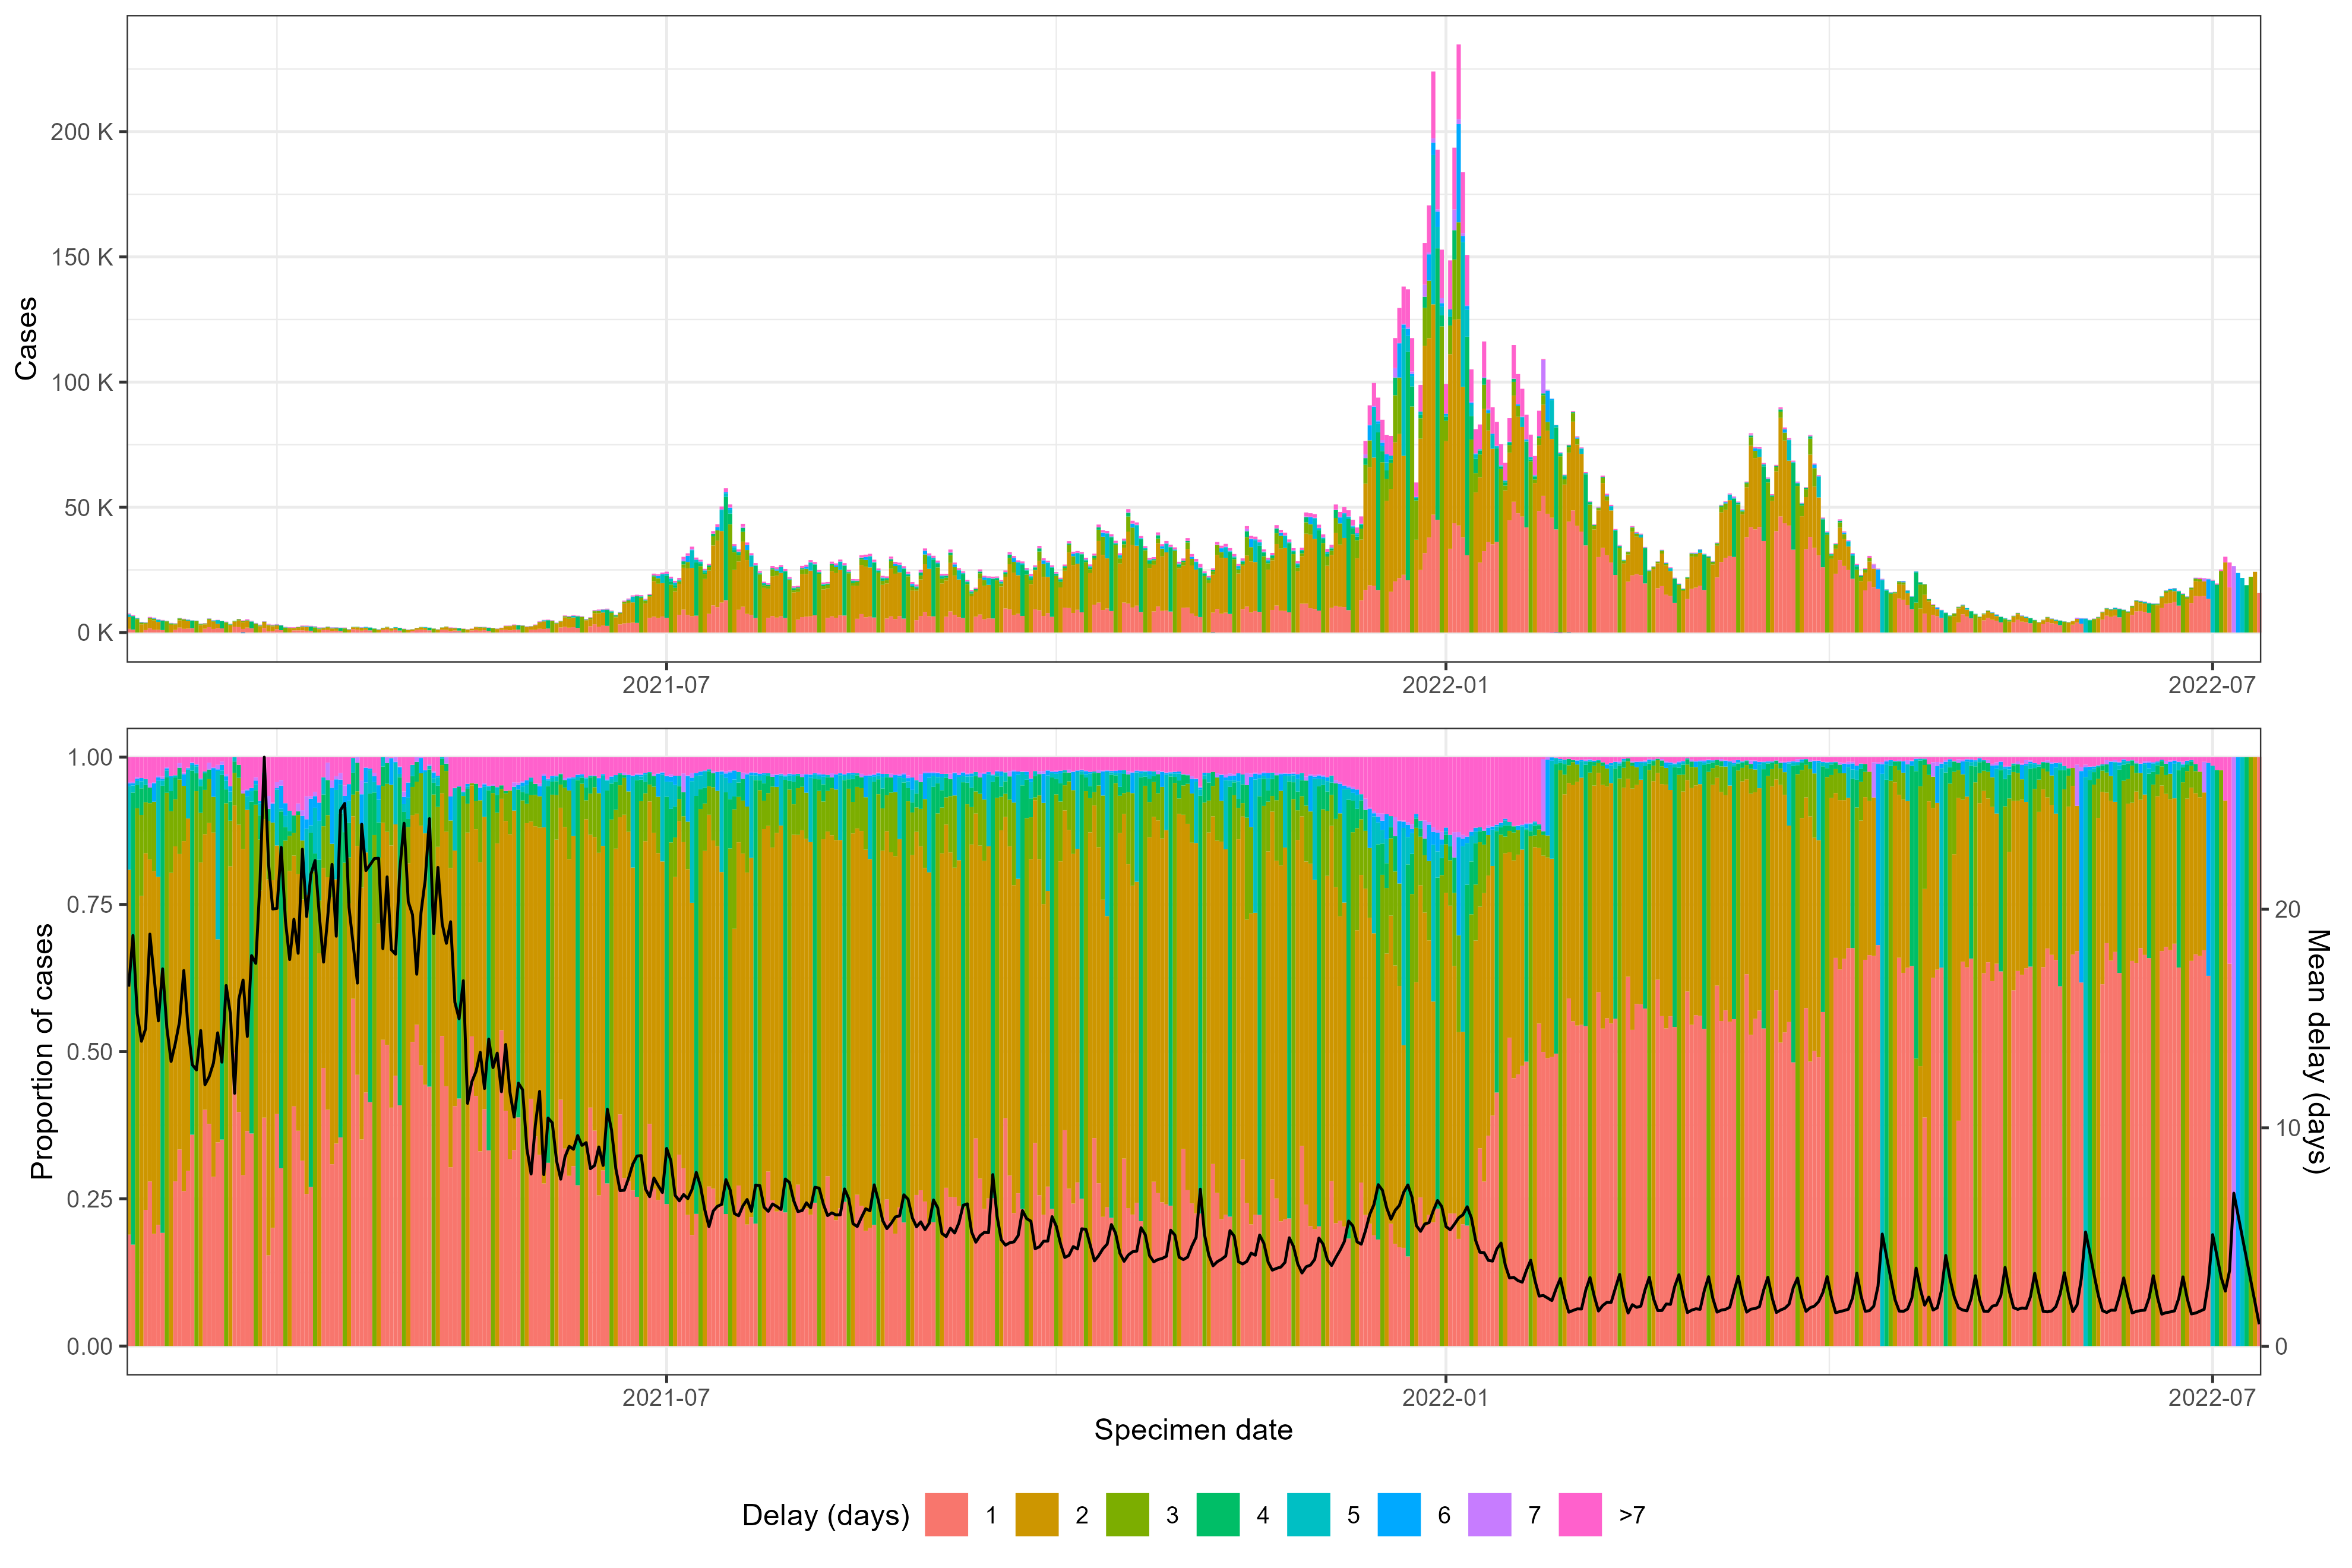
\includegraphics{images/cases-delay-england.png}

}

\caption{COVID-19 cases in England by proportion of delay}

\end{figure}

(top) New cases by specimen date. Colors represent the delay during
which cases were reported. (bottom) Proportion of new cases that are
reported by varying delays. Black line represents mean delay.

\hypertarget{long-delays}{%
\subsection{Long delays}\label{long-delays}}

\begin{itemize}
\tightlist
\item
  This section illustrates how long reporting delays can be in
  real-world data
\item
  convince reader that extra-long delays are caused by logistical issues
  rather than factors affecting transmission and can be ignored
\end{itemize}

\begin{figure}

{\centering 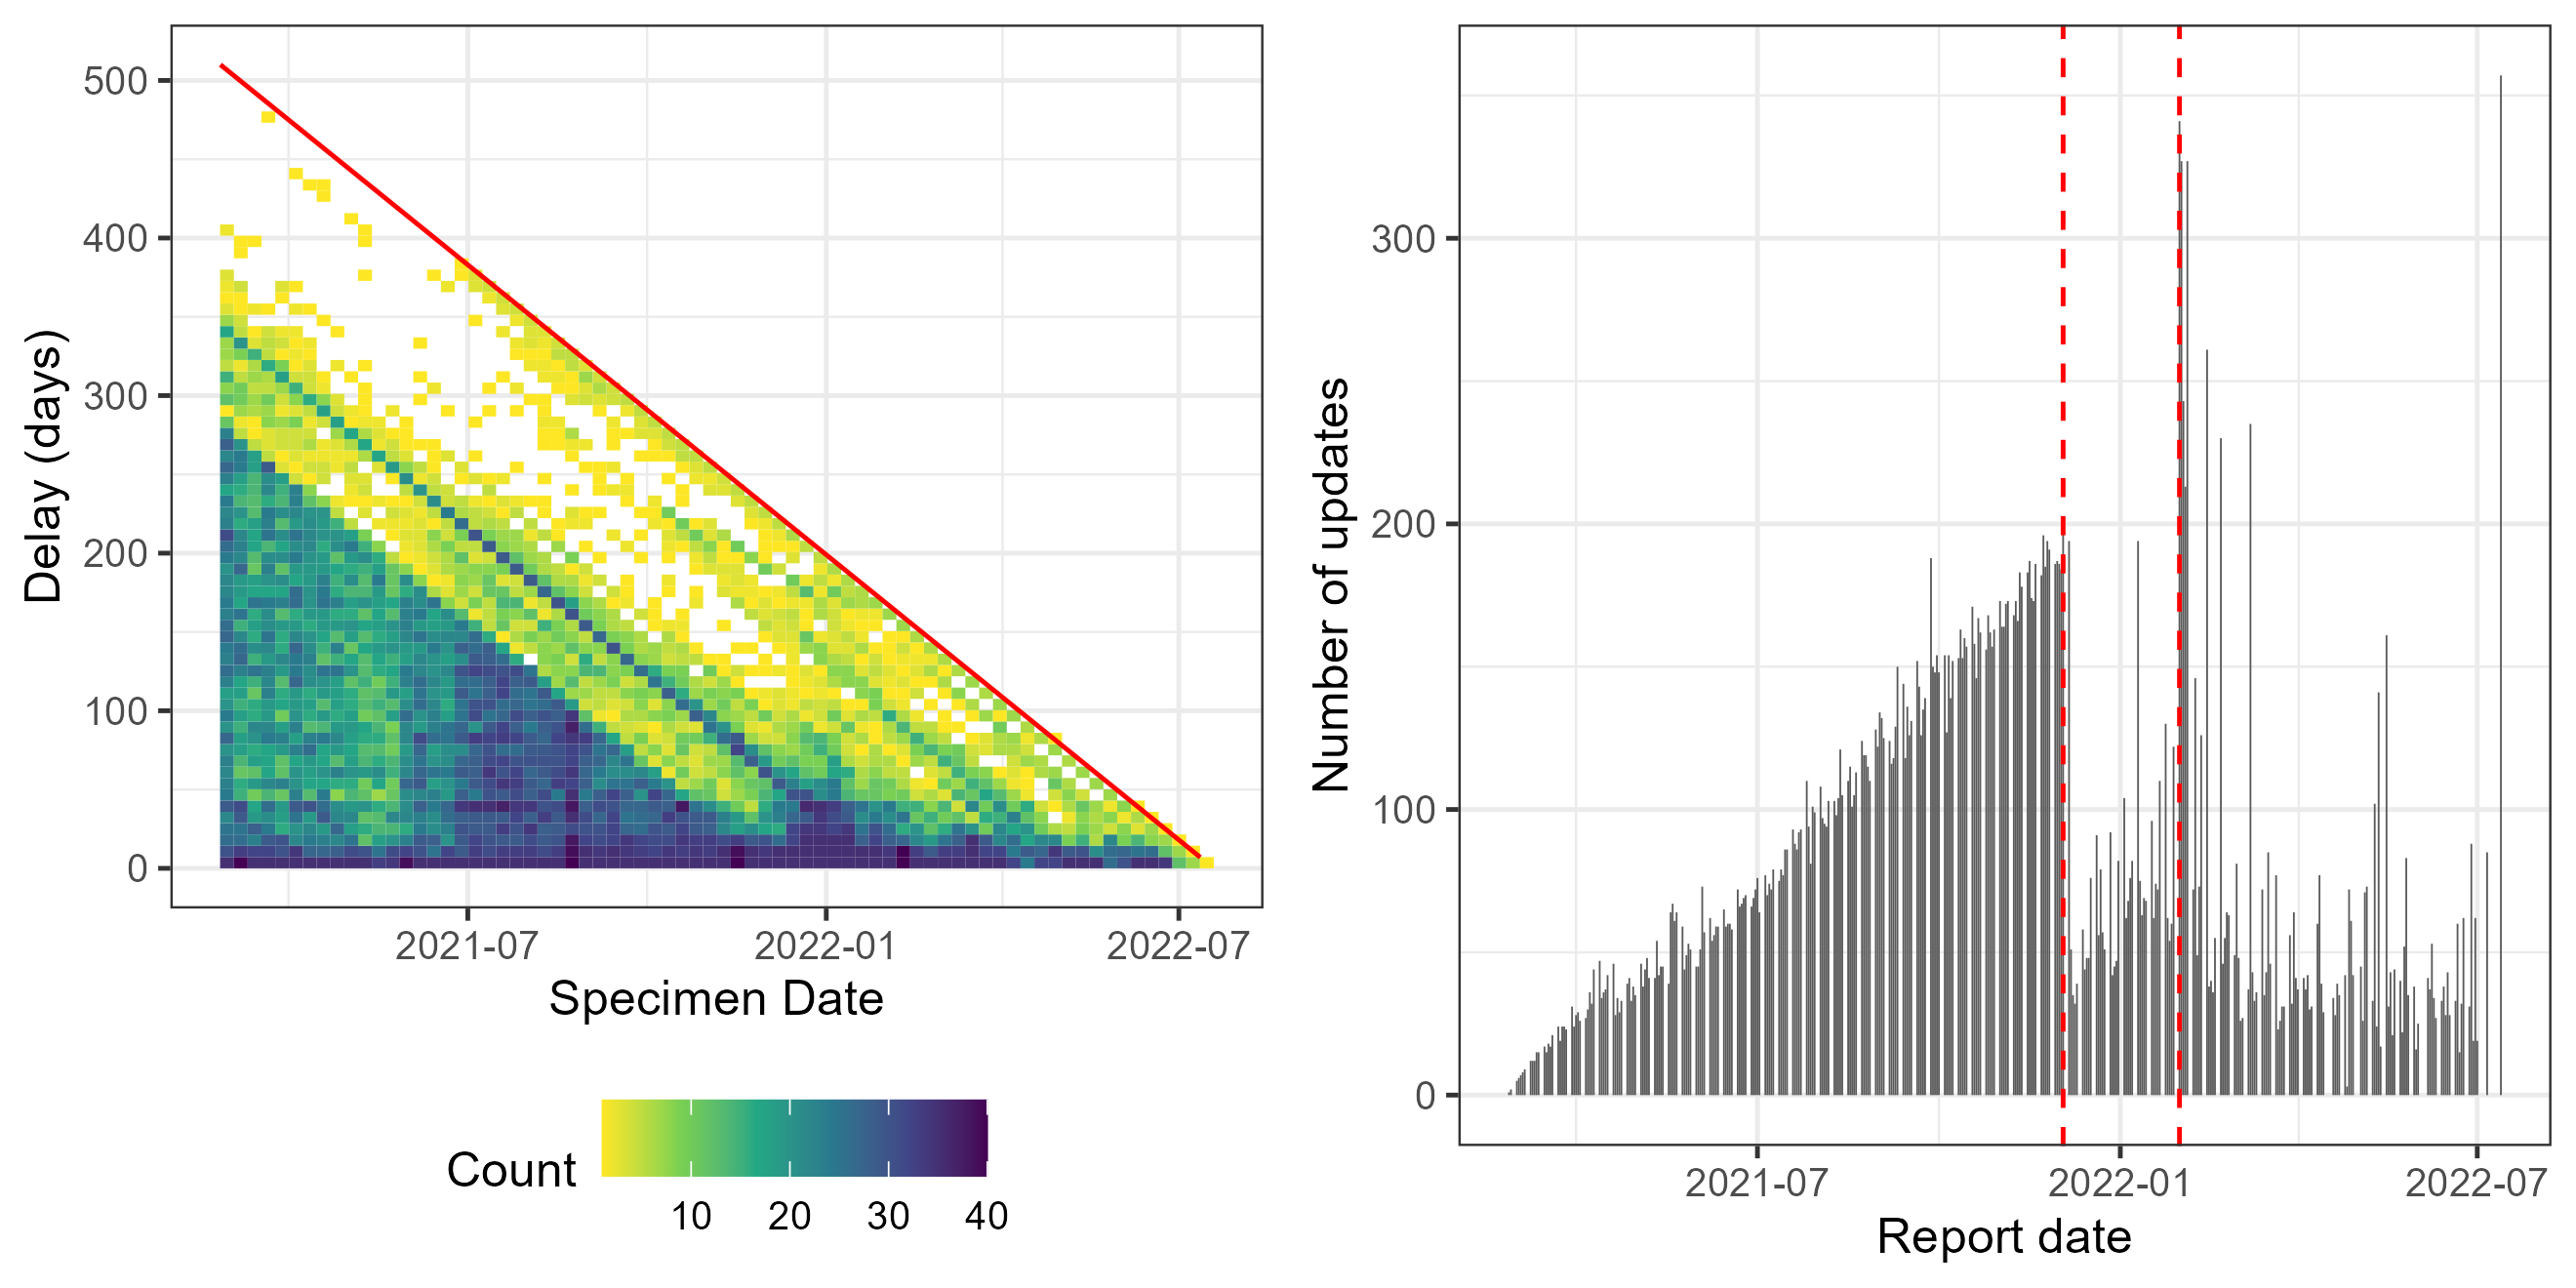
\includegraphics{images/long-delay-dist.png}

}

\caption{Distribution of long delays}

\end{figure}

(left) The frequency of updates by specimen date and delay. The hue
intensity reflects the number of updates made to the number of new cases
on each specimen date with a delay indicated by the y-axis. The red
diagonal line represents the maximum possible delay for each specimen
date. (right) The number of updates made to past data on each reporting
date. The red dotted lines represent two significant change points: the
left marks when the linearly increasing number of updates ends, and the
right highlights a particular reporting date on which there was an
unusually large number of updates made to past data.

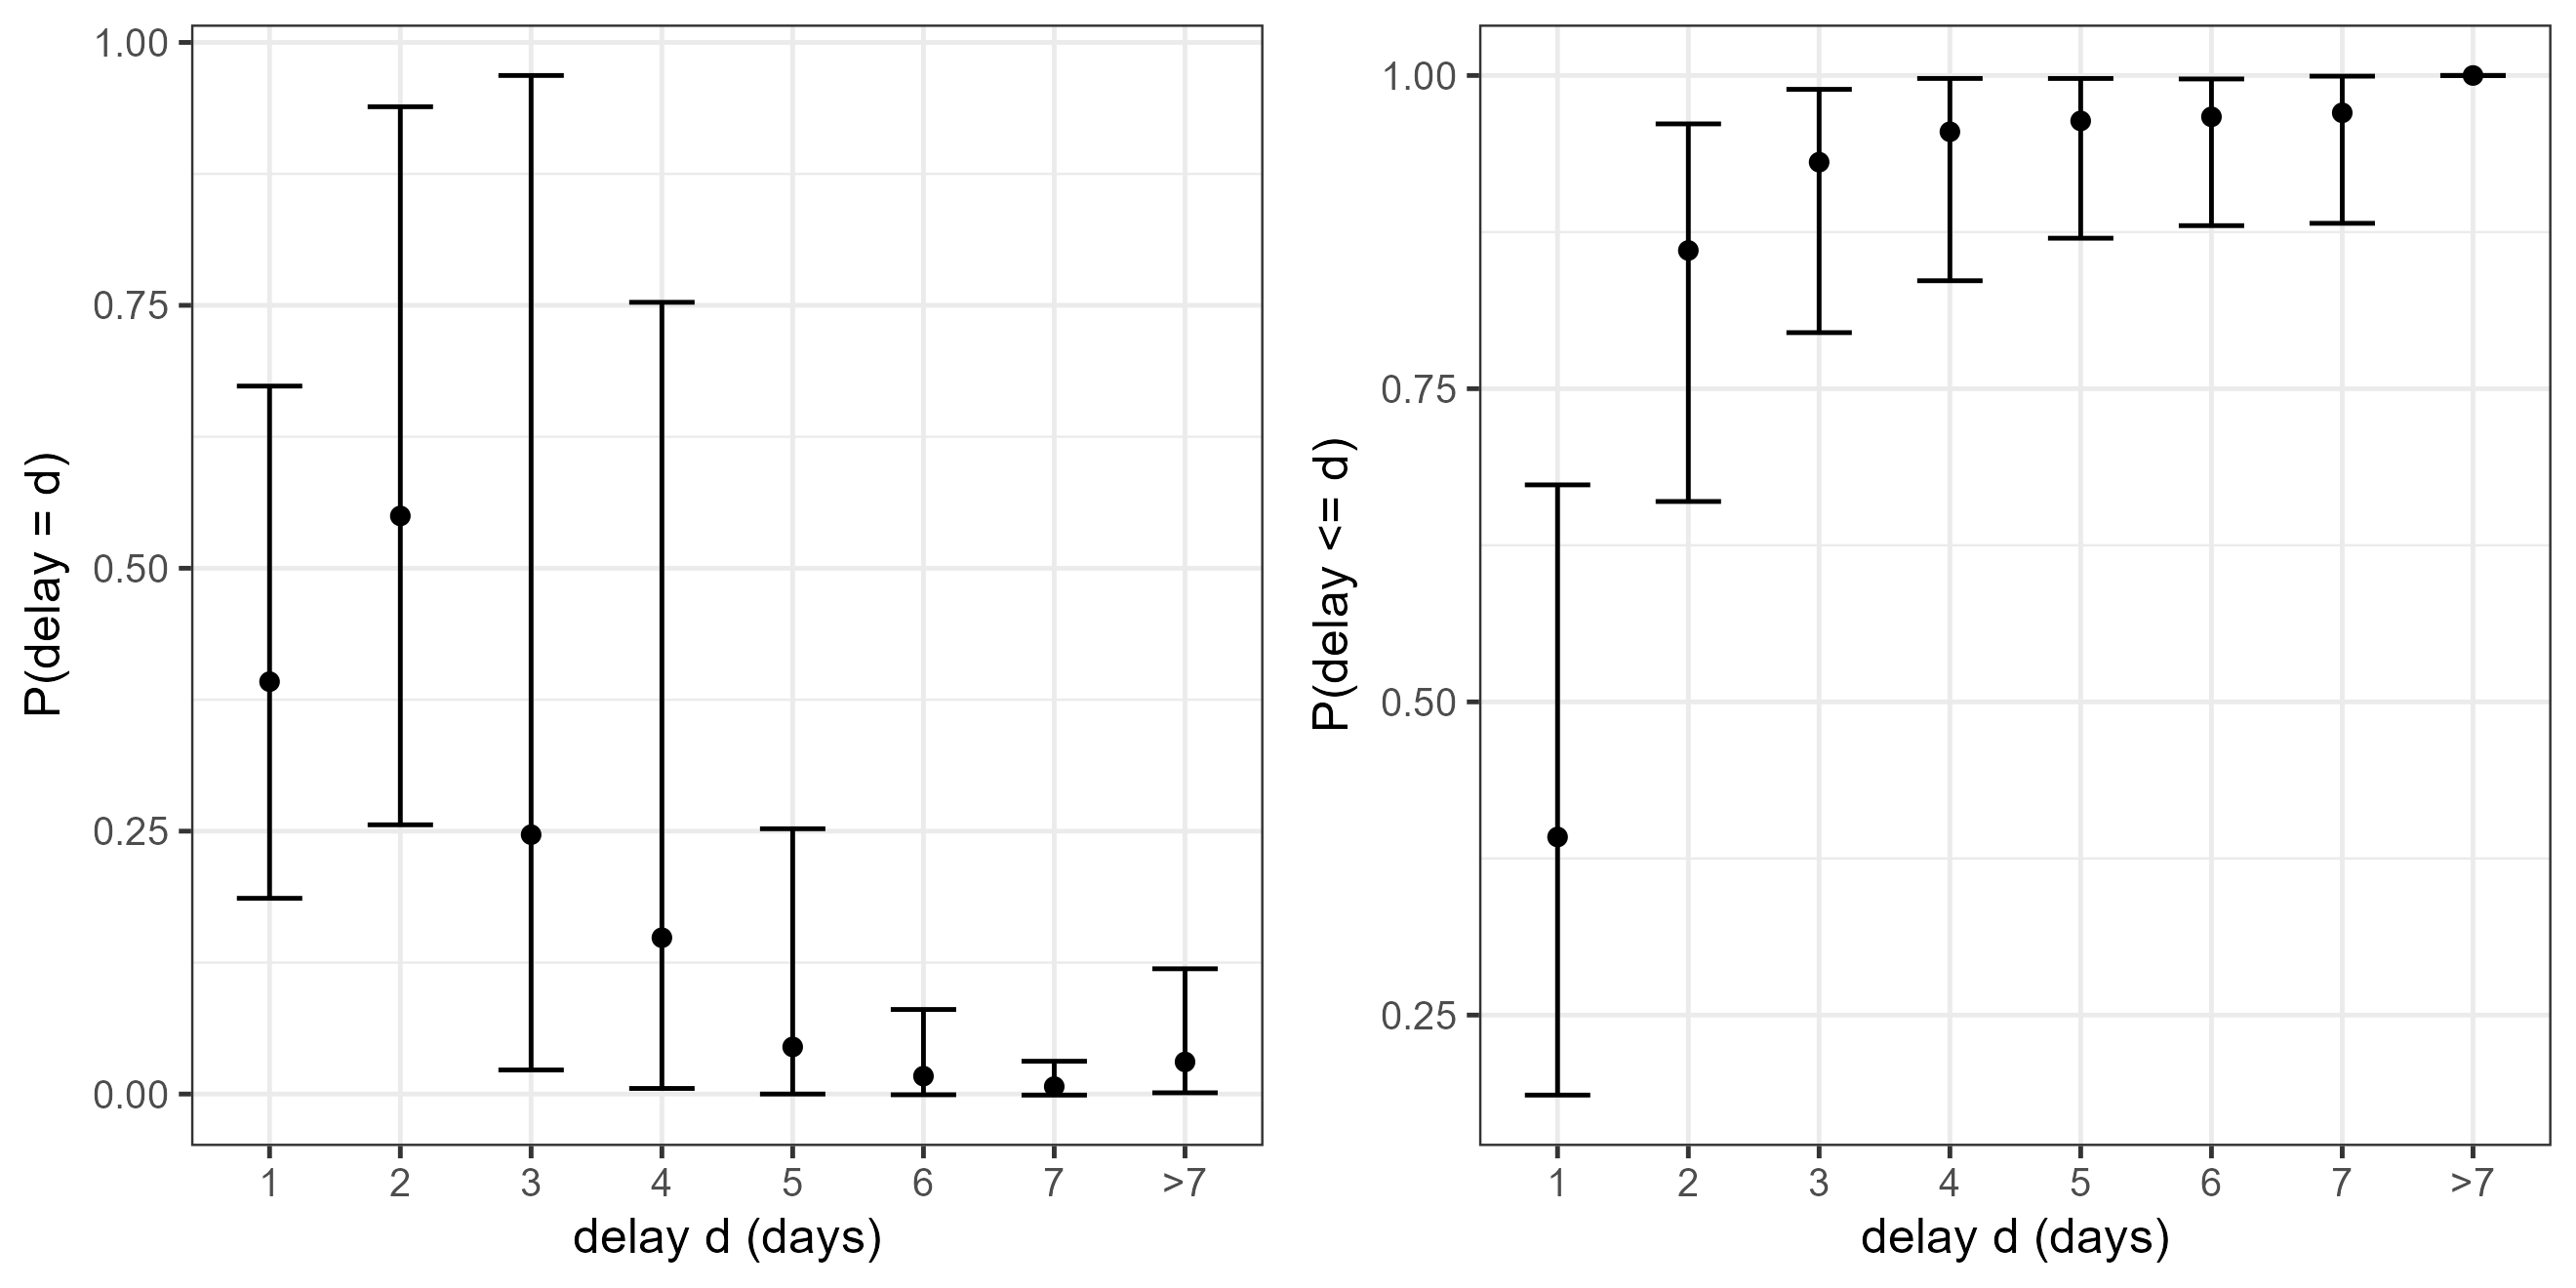
\includegraphics{images/cases-delay-dist.png} (left) The mean proportion
of cases reported with a delay \(d\) for any specimen date, with 95\%
confidence intervals. (right) The mean proportion of cases reported by a
delay \(d\) for any specimen date, with 95\% confidence intervals.

The distribution of reporting delays is right-skewed, which has a the
greatest mean proportion at \(d=2\). Cumulatively, 97.4\% of cases are
reported by day \(d=7\). This suggests that it would be practical to
take a maximum delay to be \(d>7\).

\hypertarget{test-specific-case-data}{%
\subsection{Test-specific case data}\label{test-specific-case-data}}

\begin{itemize}
\tightlist
\item
  Explain that data on new cases is the sum of three separate data
  streams
\end{itemize}

\begin{figure}

{\centering 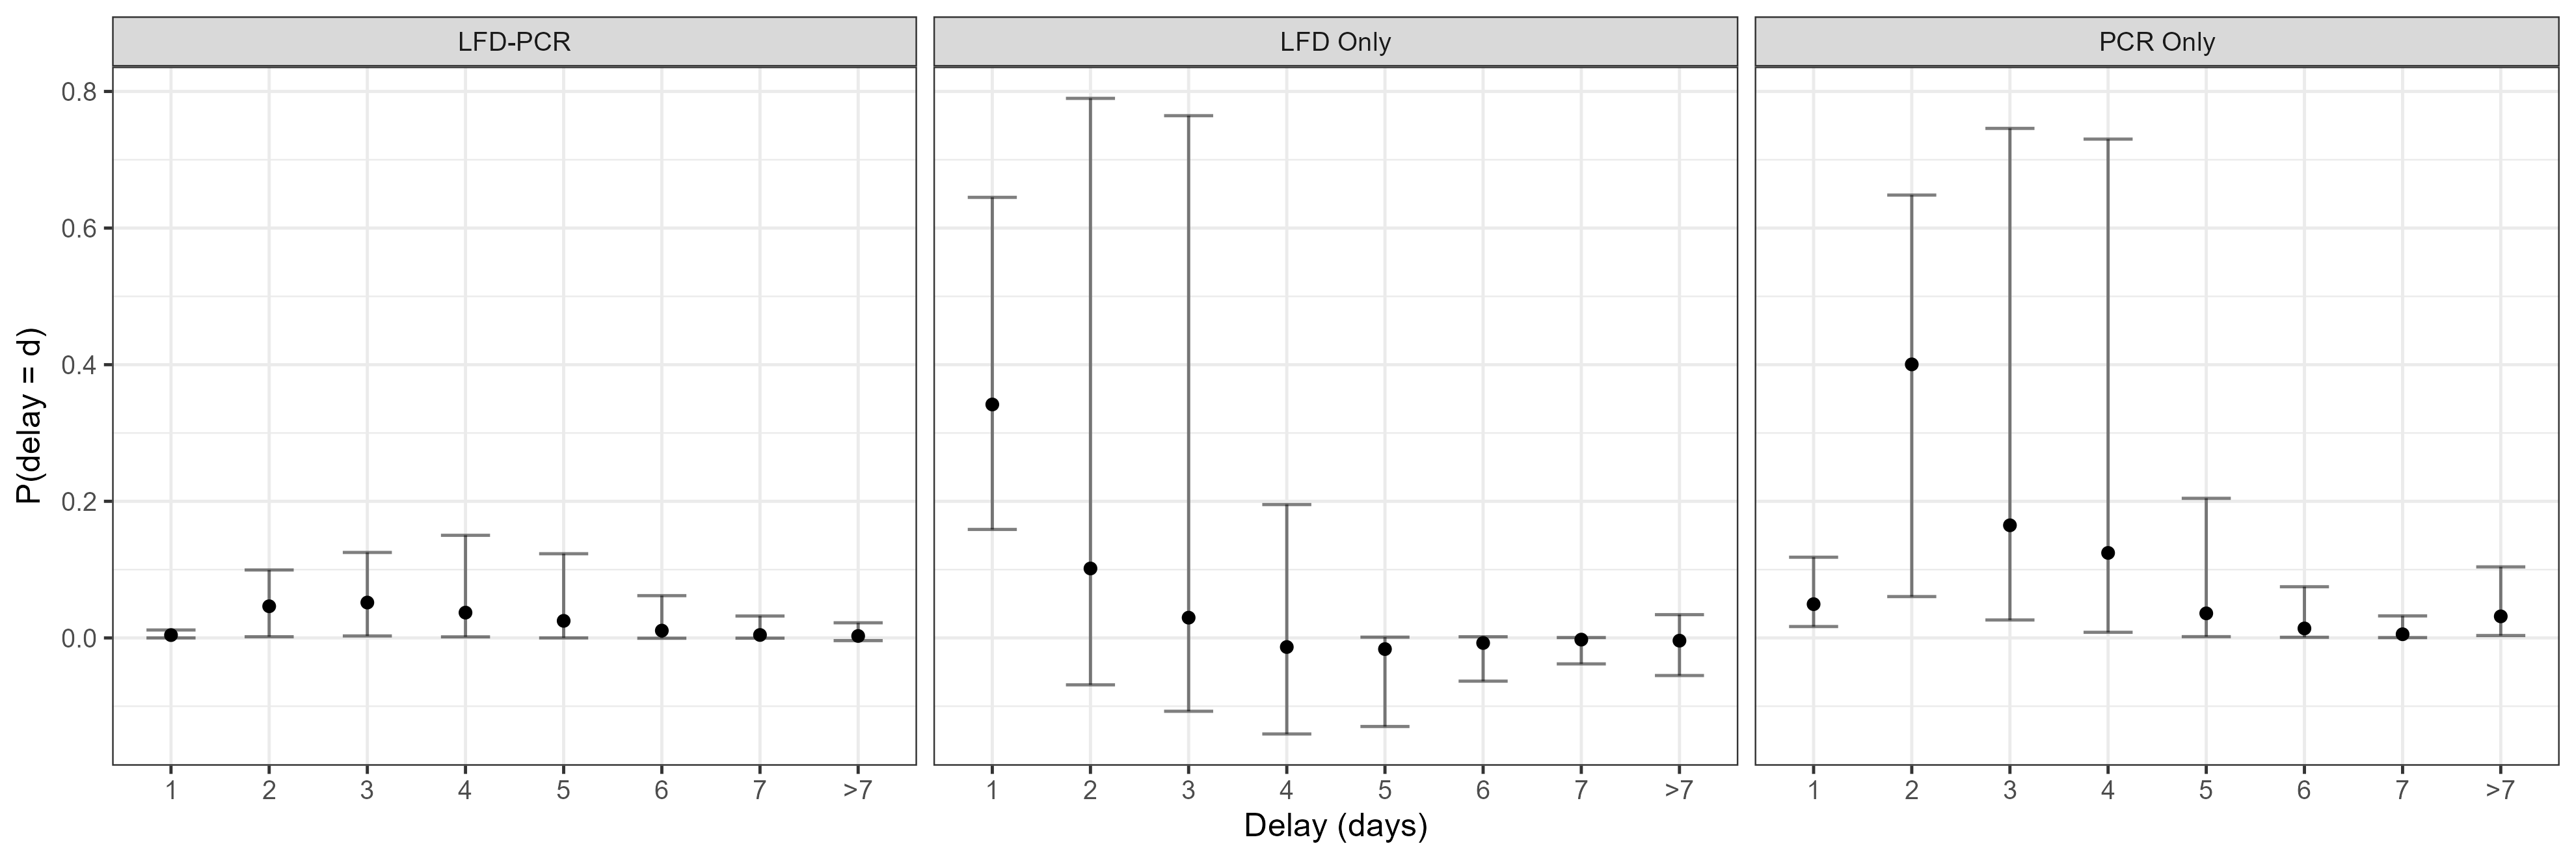
\includegraphics{images/delay-dist-test-type.png}

}

\caption{Distribution of reporting delays by test type}

\end{figure}

The majority of cases reported initially are confirmed by LFDs whilst
PCR results experience a longer lag. Due to false positives, the cases
confirmed by LFDs also update in the negative direction. Lastly, the
proportion of cases confirmed by LFD and PCR within 3 days forms the
smallest proportion of total cases reported and is slightly less right
skewed than PCR only cases. This is consistent with the understanding
that the reporting lags for both a LFD and a PCR test are expected to be
larger than just a PCR test.

\hypertarget{refs}{}
\begin{CSLReferences}{0}{0}
\leavevmode\vadjust pre{\hypertarget{ref-cox1989}{}}%
\CSLLeftMargin{{[}1{]} }%
\CSLRightInline{D. Cox and G. Medley, {``A process of events with
notification delay and the forecasting of AIDS,''} \emph{Philosophical
transactions of the Royal Society of London. Series B, Biological
sciences}, vol. 325, pp. 135--45, Oct. 1989, doi:
\href{https://doi.org/10.1098/rstb.1989.0078}{10.1098/rstb.1989.0078}.}

\leavevmode\vadjust pre{\hypertarget{ref-lawless1994}{}}%
\CSLLeftMargin{{[}2{]} }%
\CSLRightInline{J. f. Lawless, {``Adjustments for reporting delays and
the prediction of occurred but not reported events,''} \emph{Canadian
Journal of Statistics}, vol. 22, no. 1, pp. 15--31, 1994, doi:
\href{https://doi.org/10.2307/3315826.n1}{10.2307/3315826.n1}.}

\leavevmode\vadjust pre{\hypertarget{ref-huxf6hle2014}{}}%
\CSLLeftMargin{{[}3{]} }%
\CSLRightInline{M. Höhle and M. an der Heiden, {``Bayesian nowcasting
during the STEC O104:H4 outbreak in Germany, 2011,''} \emph{Biometrics},
vol. 70, no. 4, pp. 993--1002, 2014, doi:
\href{https://doi.org/10.1111/biom.12194}{10.1111/biom.12194}.}

\leavevmode\vadjust pre{\hypertarget{ref-schneble2021}{}}%
\CSLLeftMargin{{[}4{]} }%
\CSLRightInline{M. Schneble, G. De Nicola, G. Kauermann, and U. Berger,
{``Nowcasting fatal COVID-19 infections on a regional level in
Germany,''} \emph{Biometrical Journal}, vol. 63, no. 3, pp. 471--489,
2021, doi:
\href{https://doi.org/10.1002/bimj.202000143}{10.1002/bimj.202000143}.}

\leavevmode\vadjust pre{\hypertarget{ref-seaman2022}{}}%
\CSLLeftMargin{{[}5{]} }%
\CSLRightInline{S. R. Seaman, P. Samartsidis, M. Kall, and D. De
Angelis, {``Nowcasting COVID-19 deaths in England by age and region,''}
\emph{Journal of the Royal Statistical Society: Series C (Applied
Statistics)}, vol. n/a, no. n/a, Jun. 2022, doi:
\href{https://doi.org/10.1111/rssc.12576}{10.1111/rssc.12576}.}

\leavevmode\vadjust pre{\hypertarget{ref-abbott2021}{}}%
\CSLLeftMargin{{[}6{]} }%
\CSLRightInline{S. Abbott, \emph{Epinowcast: Hierarchical nowcasting of
right censored epidemological counts}. 2021.}

\leavevmode\vadjust pre{\hypertarget{ref-guxfcnther2021}{}}%
\CSLLeftMargin{{[}7{]} }%
\CSLRightInline{F. Günther, A. Bender, K. Katz, H. Küchenhoff, and M.
Höhle, {``Nowcasting the COVID-19 pandemic in Bavaria,''}
\emph{Biometrical Journal}, vol. 63, no. 3, pp. 490--502, 2021, doi:
\href{https://doi.org/10.1002/bimj.202000112}{10.1002/bimj.202000112}.}

\leavevmode\vadjust pre{\hypertarget{ref-rcoreteam2022}{}}%
\CSLLeftMargin{{[}8{]} }%
\CSLRightInline{R Core Team, \emph{R: A language and environment for
statistical computing}. Vienna, Austria: R Foundation for Statistical
Computing, 2022. Available: \url{https://www.R-project.org/}}

\leavevmode\vadjust pre{\hypertarget{ref-gneiting2007}{}}%
\CSLLeftMargin{{[}9{]} }%
\CSLRightInline{T. Gneiting and A. E. Raftery, {``Strictly proper
scoring rules, prediction, and estimation,''} \emph{Journal of the
American Statistical Association}, vol. 102, no. 477, pp. 359--378, Mar.
2007, doi:
\href{https://doi.org/10.1198/016214506000001437}{10.1198/016214506000001437}.}

\leavevmode\vadjust pre{\hypertarget{ref-bracher2021}{}}%
\CSLLeftMargin{{[}10{]} }%
\CSLRightInline{J. Bracher, E. L. Ray, T. Gneiting, and N. G. Reich,
{``Evaluating epidemic forecasts in an interval format,''} \emph{PLOS
Computational Biology}, vol. 17, no. 2, p. e1008618, Feb. 2021, doi:
\href{https://doi.org/10.1371/journal.pcbi.1008618}{10.1371/journal.pcbi.1008618}.}

\leavevmode\vadjust pre{\hypertarget{ref-bosse}{}}%
\CSLLeftMargin{{[}11{]} }%
\CSLRightInline{N. I. Bosse, H. Gruson, A. Cori, E. van Leeuwen, S.
Funk, and S. Abbott, {``Evaluating forecasts with scoringutils in r,''}
doi:
\href{https://doi.org/10.48550/arXiv.2205.07090}{10.48550/arXiv.2205.07090}.}

\end{CSLReferences}



\end{document}
